\documentclass{standalone}
\usepackage{tikz}
\usepackage{amsmath}
\usepackage{amsfonts}
\usepackage{cellspace}
\usepackage{pgfplots}
\usepackage{array}

\begin{document} 
\newcommand\braingraphic[2][]{\raisebox{-0.5\height}{\includegraphics[width=6cm, height=4.4cm]{#2}}}

\pgfmathdeclarefunction{gauss}{2}{%
	\pgfmathparse{1/(#2*sqrt(2*pi))*exp(-((x-#1)^2)/(2*#2^2))}%
}

\begin{tabular}{ >{\centering}m{9cm} | c }
	Gender is a binary set of $\{male, female\}$ &
	\braingraphic{0.jpg} \\
	
	\hline
	
	Gender is a bimodal distribution on a spectrum that is isomorphic to the set of real numbers $\mathbb{R}$ 
	
	\begin{tikzpicture}
		\begin{axis}[height=4cm]
			\addplot[color=red, samples=300]{0.5 * (gauss(-2, 0.8) + gauss(2, 0.8))};
		\end{axis}
	\end{tikzpicture} &
	\braingraphic{1.jpg} \\
	\hline
	
	Gender is a 2D plane isomorphic to $\mathbb{R}^2$ where individual genders $(m, f) \in \text{Gender}$ encode masculinity and femininity as a 2-vector 
	
	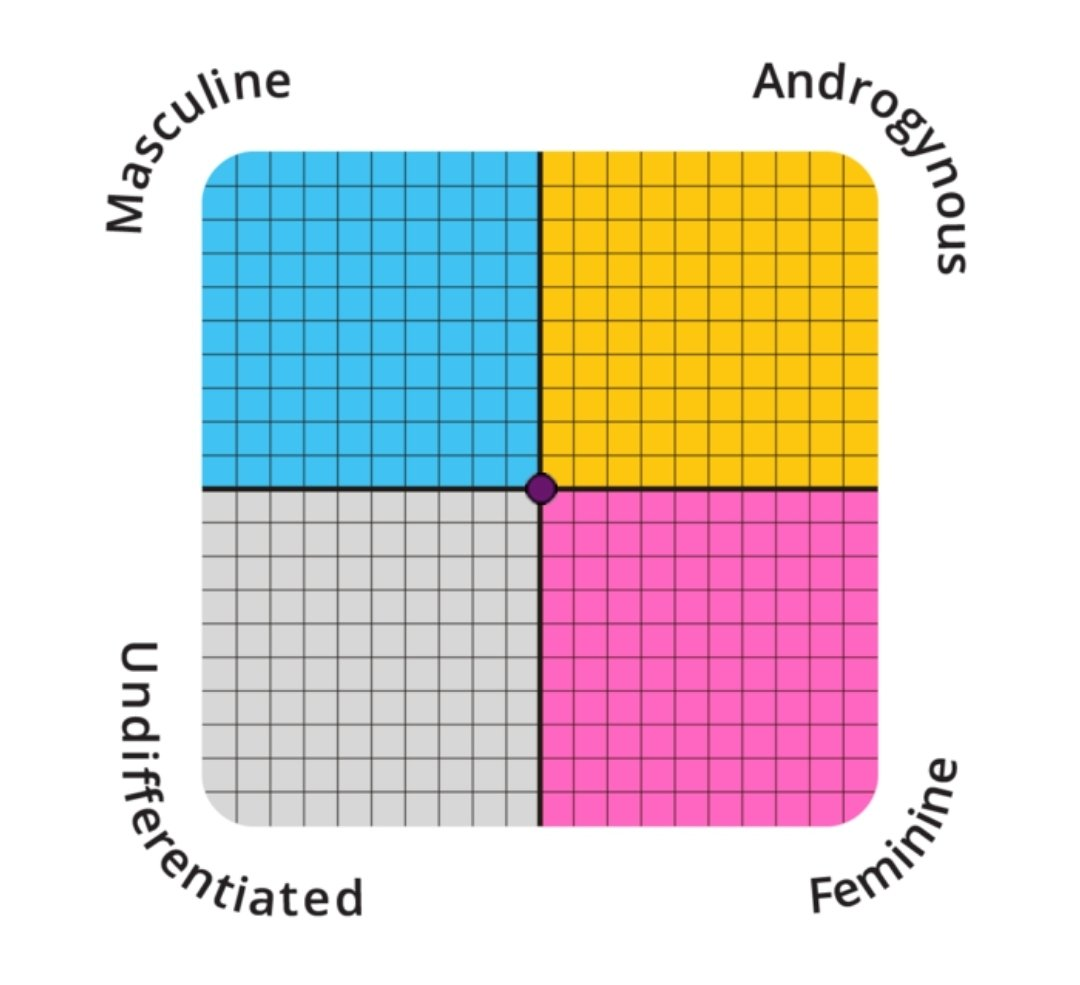
\includegraphics[width=3cm, height=3cm]{2d.jpg}&
	\braingraphic{2.jpg} \\
	\hline
			
	Gender is a $n$-dimensional vector space isomorphic to $\mathbb{R}^n$ where individual genders 
	$$(m, f, x_3, x_4, \dots, x_n) \in \text{Gender}$$
	encode masculinity, femininity, and $n - 2$ dimensions of xenogenders
	
	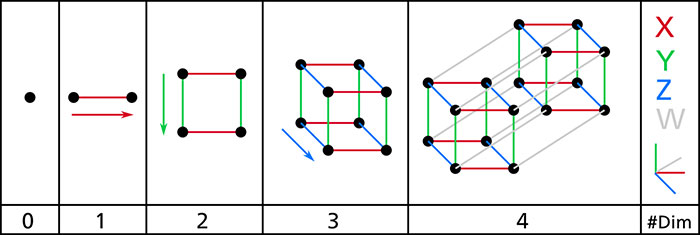
\includegraphics[width=5cm, height=1cm]{nd.jpg}
    &
	\braingraphic{3.jpg} \\
	\hline
	
	Gender is a vector-valued function 
	$$g(t) = (m, f, x_3, x_4, \dots, x_n)$$
	encoding a 1-dimensional nonlinear and possibly cyclical path over time through the $n$-dimensional hyperspace of all static genders
	 
	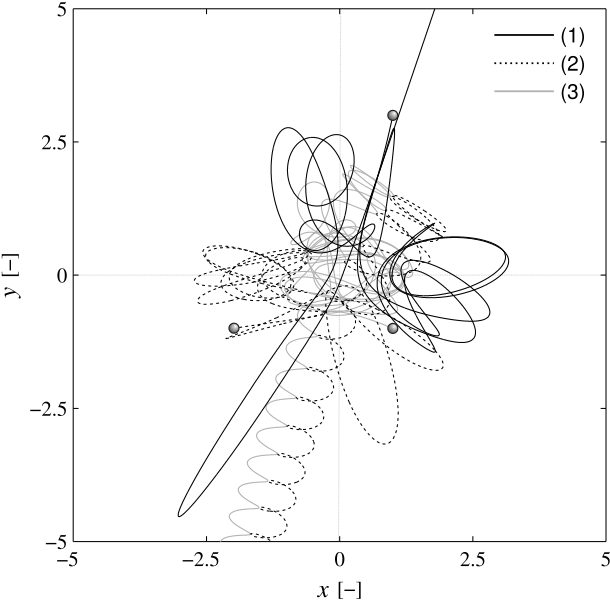
\includegraphics[width=5cm, height=2cm]{path.png}&
	\braingraphic{4.jpg} \\
	\hline
	
	Gender is hard and I don't wanna think about it ;-; &
	\braingraphic{5.jpg}  \\
	\hline
made in \LaTeX out of boredom
\end{tabular} 
\end{document}